\documentclass[aspectratio=169,11pt]{beamer}
\usepackage{lmodern}
\usetheme[progressbar=frametitle,numbering=fraction]{metropolis}
\usepackage{amsmath,amssymb,bm}
\usepackage{listings,xcolor}
\usepackage{booktabs}
\definecolor{given}{HTML}{1F6FB2}
\definecolor{hand}{HTML}{2E7D32}
\definecolor{algo}{HTML}{B26A00}
\definecolor{impl}{HTML}{6A1B9A}
\lstset{language=Python,basicstyle=\ttfamily\footnotesize,keywordstyle=\color{impl}\bfseries,
  commentstyle=\color{gray},showstringspaces=false,columns=fullflexible,keepspaces=true}
% stage labels: every solution slide says which stage it is
\newcommand{\stage}[2]{{\color{#1}\bfseries\small\textsc{#2}}\par\smallskip}
\newcommand{\Byhand}{\stage{hand}{Step 1 -- by hand}}
\newcommand{\Algo}{\stage{algo}{Step 2 -- algorithm}}
\newcommand{\Impl}{\stage{impl}{Step 3 -- implementation}}
\newcommand{\Given}{\stage{given}{Recap}}
\newcommand{\Refresh}{\stage{given}{Refresher}}
\title{Exercise 2 -- Problem 2.3: fitting a Weibull to a histogram (part 2)}
\subtitle{Principles of Machine Learning (MA-INF 4111), WS 2026/27}
\date{Solution slides}
\begin{document}
\maketitle

\begin{frame}{Roadmap}
\begin{enumerate}
\item \textbf{Refresher}: least squares, and why a pdf needs an amplitude to match counts
\item \textbf{Recap of the task}: what is given, what we must do
\item \textbf{Task 2.3.1}: fit $A\,f(t\mid\alpha,\beta)$ with \texttt{curve\_fit()}
\item \textbf{Task 2.3.2}: plot the fit, and see why it differs from Problem 2.2
\end{enumerate}
\bigskip
Every solution follows the same three steps:\\[3pt]
\textcolor{hand}{\textbf{by hand}} \;$\to$\; \textcolor{algo}{\textbf{algorithm}} \;$\to$\; \textcolor{impl}{\textbf{implementation}}
\end{frame}

% =====================================================================
\section{Refresher: what you should remember}

\begin{frame}{Refresher: least squares, step by step}
\Refresh
Data points $(t_i,y_i)$, $i=1,\dots,n$; a model curve $m(t\mid\bm\theta)$ with parameters $\bm\theta$.
\begin{enumerate}
\item \textbf{Residual} of point $i$: \quad $r_i(\bm\theta)=y_i-m(t_i\mid\bm\theta)$ \quad (vertical distance)
\item \textbf{Sum of squared residuals}:
\[S(\bm\theta)=\sum_{i=1}^n r_i(\bm\theta)^2\]
\item \textbf{Least squares}: choose $\hat{\bm\theta}=\arg\min_{\bm\theta} S(\bm\theta)$
\end{enumerate}
\medskip
Squares: positive and negative errors do not cancel, $S$ is differentiable, and large errors are punished most.\\
If $m$ is \textbf{linear} in $\bm\theta$: set $\nabla S=0$, closed form. If not: iterate.
\end{frame}

\begin{frame}{Refresher: a pdf does not have the size of the counts}
\Refresh
\begin{enumerate}
\item A pdf has area $1$. With bins of width $1$: \quad $\sum_{t=1}^n f(t\mid\alpha,\beta)\approx1$
\item The counts add up to \quad $C=\sum_{t=1}^n c_t=17293$
\item So $f$ alone is far too small to lie on the data. A count curve needs a factor:
\[c_t\approx A\cdot f(t\mid\alpha,\beta),\qquad A\approx C\]
\item In 2.2 we fixed $A=C$ \emph{after} the fit. Now $A$ becomes a \textbf{third parameter}.
\end{enumerate}
\end{frame}

% =====================================================================
\section{Recap of the task}

\begin{frame}{Given}
\Given
\begin{itemize}
\item Data from 2.1: counts $\bm c=[c_1,\dots,c_n]$, weeks $\bm t=[1,\dots,n]$, $n=453$
\item Weibull pdf (3):\quad
$f(t\mid\alpha,\beta)=\dfrac{\alpha}{\beta}\Big(\dfrac t\beta\Big)^{\alpha-1}\exp\!\Big[-\Big(\dfrac t\beta\Big)^{\alpha}\Big]$,\quad $\alpha,\beta>0$
\item Our \texttt{weibull\_pdf(t, alpha, beta)} from 2.1.2
\item Result of 2.2 (Newton / MLE): $\hat\alpha=2.809$, $\hat\beta=215.43$
\item \texttt{scipy.optimize.curve\_fit(f, xdata, ydata, p0, bounds)}: least squares fit of a curve to points
\end{itemize}
\end{frame}

\begin{frame}{Problem to solve}\small
\Given
\begin{description}[Task 2.3.2]
\item[Task 2.3.1] Fit the \textbf{scaled Weibull}
\[\tilde f(t\mid A,\alpha,\beta)=A\cdot f(t\mid\alpha,\beta)\qquad(11)\]
to $(\bm t,\bm c)$ with \texttt{curve\_fit()}. Initial guesses (12): $\alpha=2$, $\beta=200$, $A=1000$.
Tell \texttt{curve\_fit()} that $\alpha,\beta$ must be \textbf{positive} (bounds). Report $\hat\alpha,\hat\beta$.
\item[Task 2.3.2] Plot the fitted model together with the data.
\end{description}
\medskip
The sheet warns: (a) this is a \emph{hack}, (b) the result will \emph{not} equal 2.2. We explain both.
\end{frame}

% =====================================================================
\section{Task 2.3.1: fit with \texttt{curve\_fit()}}

\begin{frame}{2.3.1 -- what exactly is minimised?}
\Byhand
\texttt{curve\_fit} treats the counts as \textbf{points on a curve}, $y_t=c_t$, and minimises
\[
S(A,\alpha,\beta)=\sum_{t=1}^{n}\Big(c_t-A\,f(t\mid\alpha,\beta)\Big)^2
\]
\begin{itemize}
\item Three unknowns: $A$ (height), $\alpha$ (shape), $\beta$ (scale)
\item $S$ is \textbf{linear in $A$} but \textbf{nonlinear in $\alpha,\beta$} $\Rightarrow$ no closed form, iterate
\item Each \emph{week} counts once. Nothing here uses that $f$ is a probability density\\
$\Rightarrow$ the ``hack'': statistically, MLE (2.2) is the principled choice
\end{itemize}
\end{frame}

\begin{frame}{2.3.1 -- by hand: the best amplitude for a fixed shape}\small
\Byhand
Fix $\alpha,\beta$ and write $g_t=f(t\mid\alpha,\beta)$. Then $S(A)=\sum_t(c_t-Ag_t)^2$ is a parabola in $A$:
\[
\frac{\mathrm dS}{\mathrm dA}=-2\sum_t g_t\,(c_t-Ag_t)=0
\quad\Longrightarrow\quad
A^*=\frac{\sum_t c_tg_t}{\sum_t g_t^2}
\]
\textbf{Toy:} $\bm g=[0.25,\,0.5,\,0.25]$ (sums to 1), $\bm c=[2,\,4,\,3]$ (sums to 9).
\begin{enumerate}
\item $\sum c_tg_t=0.5+2+0.75=3.25$,\quad $\sum g_t^2=0.0625+0.25+0.0625=0.375$
\item $A^*=3.25/0.375=8.67$ \quad (close to $\sum c_t=9$, but not equal)
\item Residuals: $2-2.17=-0.17$,\; $4-4.33=-0.33$,\; $3-2.17=0.83$\quad$\Rightarrow S=0.83$
\end{enumerate}
\alert{Lesson:} $A$ is ``roughly the total count'', adjusted to fit the points best.
\end{frame}

\begin{frame}{2.3.1 -- by hand: the start (12) on the real data}
\Byhand
\begin{columns}[T]
\column{.42\textwidth}\small
\begin{itemize}
\item Start $A=1000,\alpha=2,\beta=200$:\\ curve peaks near $4$, data near $100$\\
$S=1\,042\,660$
\item Keep the shape, take the best $A$ (formula on the last slide):\\
$A^*=18\,331$, \quad $S=101\,626$
\item $A^*$ is close to $C=17\,293$: the amplitude is the easy part
\item What is left is the \textbf{shape}: $\alpha,\beta$
\end{itemize}
\column{.56\textwidth}
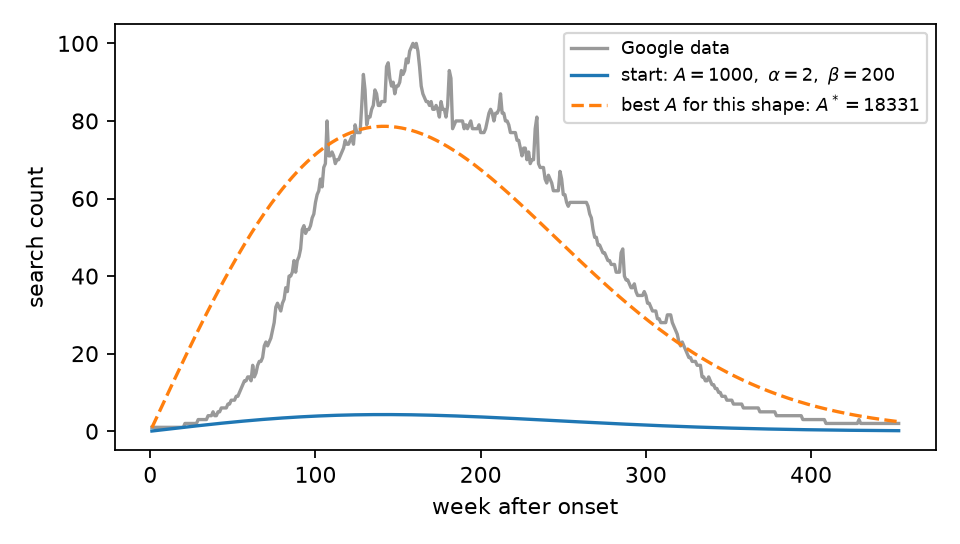
\includegraphics[width=\linewidth]{figures/start_guess.png}
\end{columns}
\end{frame}

\begin{frame}[fragile]{2.3.1 -- by hand: why the bounds are critical}
\Byhand
Try a step that overshoots to $\beta=-200$ with $\alpha=2.5$, at $t=100$:
\[
\Big(\frac{t}{\beta}\Big)^{\alpha-1}=(-0.5)^{1.5}=\;?\qquad\text{(no real number)}
\]
\begin{lstlisting}
>>> weibull_pdf(np.array([1., 100.]), 2.5, -200)
array([nan, nan])
\end{lstlisting}
\begin{itemize}
\item One \texttt{nan} in the residuals and the optimiser is lost
\item The optimiser does \textbf{not} know that $\alpha,\beta>0$: we must tell it
\item Lower bound $10^{-6}$, not $0$: $\beta=0$ divides by zero
\end{itemize}
\end{frame}

\begin{frame}{2.3.1 -- algorithm}\footnotesize
\Algo
\textbf{Input:} $\bm t,\bm c$, model $\tilde f$, start $\bm\theta_0=(A,\alpha,\beta)=(1000,2,200)$, bounds $\bm\theta>0$
\begin{enumerate}
\item Residual vector $\bm r(\bm\theta)=\bm c-\tilde f(\bm t\mid\bm\theta)\in\mathbb R^{n}$
\item Jacobian $J=\partial\bm r/\partial\bm\theta\in\mathbb R^{n\times3}$ (\texttt{curve\_fit}: finite differences)
\item Linearise $\bm r(\bm\theta+\bm\delta)\approx\bm r+J\bm\delta$ and solve the small least squares problem
\[\min_{\bm\delta}\ \|\bm r+J\bm\delta\|^2 \quad\text{(inside a trust region)}\]
\item Keep the step only if $S$ decreases and $\bm\theta+\bm\delta$ stays inside the bounds
\item Repeat until $S$ hardly changes (here: 23 evaluations)
\end{enumerate}
With bounds, \texttt{curve\_fit} uses the \emph{trust region reflective} method (\texttt{'trf'}),\\
without bounds Levenberg--Marquardt. Both are this Gauss--Newton idea plus safeguards.
\end{frame}

\begin{frame}[fragile]{2.3.1 -- implementation}
\Impl
\begin{lstlisting}
from scipy.optimize import curve_fit

def scaled_weibull(t, A, alpha, beta):      # model (11)
    return A * weibull_pdf(t, alpha, beta)

t, c = load_myspace_data()
p0     = [1000.0, 2.0, 200.0]                         # (12): A, alpha, beta
bounds = ([0.0, 1e-6, 1e-6], [np.inf, np.inf, np.inf]) # lower, upper
popt, pcov = curve_fit(scaled_weibull, t, c, p0=p0, bounds=bounds)
A, alpha, beta = popt
\end{lstlisting}
\footnotesize
\begin{itemize}
\item Order of \texttt{p0} and \texttt{bounds} $=$ order of the arguments \emph{after} \texttt{t}: \texttt{(A, alpha, beta)}
\item \texttt{bounds} is a pair \texttt{(lower, upper)}, one entry per parameter
\end{itemize}
\end{frame}

\begin{frame}{2.3.1 -- result and checks}
\Impl
\[
\boxed{\hat\alpha\approx2.731,\qquad\hat\beta\approx211.02,\qquad\hat A\approx17\,459}
\qquad S=13\,153
\]
\textbf{Checks}
\begin{itemize}
\item Other starts $(5000,1.5,100)$ and $(20000,3,250)$: same optimum to 6 digits
\item $\hat A/C=17459/17293=1.0096$: the amplitude is the total count, as expected
\item The MLE fit of 2.2 (scaled by $C$) has $S=15\,543>13\,153$: least squares wins \emph{its own} criterion
\item A bad start $(1,1,1)$ fails (``maximum number of function evaluations exceeded''):\\
$S$ is not convex, which is why the sheet hands us (12)
\end{itemize}
\end{frame}

% =====================================================================
\section{Task 2.3.2: plot, and compare with 2.2}

\begin{frame}[fragile]{2.3.2 -- plot the fitted model}
\Impl
\begin{columns}[T]
\column{.42\textwidth}
\begin{lstlisting}
plt.plot(t, c, label="Google data")
plt.plot(t, scaled_weibull(t, *popt),
         label="Weibull fit")
plt.legend()
\end{lstlisting}
\small
\begin{itemize}
\item No extra scaling: $\hat A$ is part of the model
\item Looks like the instructor's figure (sheet p.~10)
\end{itemize}
\column{.56\textwidth}
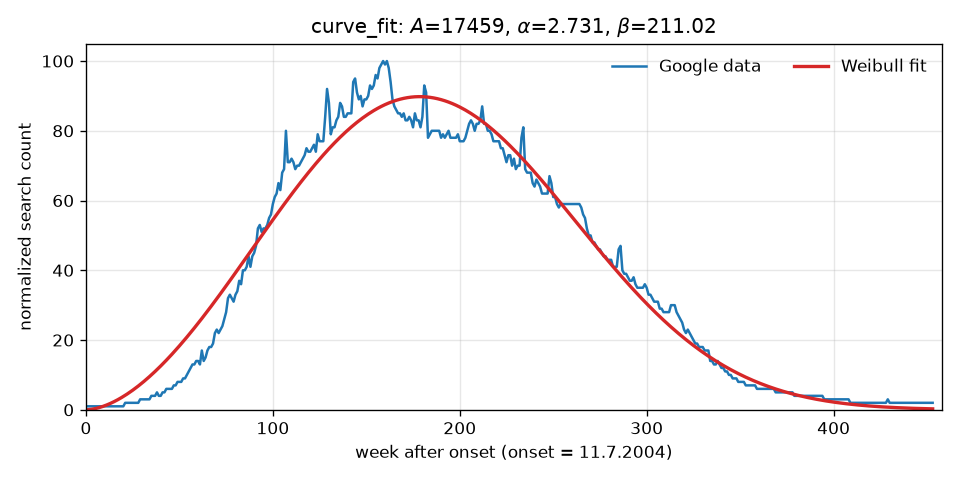
\includegraphics[width=\linewidth]{figures/task_2_3_2_curve_fit.png}
\end{columns}
\end{frame}

\begin{frame}{Why is the result not the same as in 2.2?}
\begin{center}
\begin{tabular}{lcc}
\toprule
& 2.2 Newton / MLE & 2.3 least squares\\
\midrule
objective & maximise $\sum_t c_t\log f(t)$ & minimise $\sum_t\big(c_t-Af(t)\big)^2$\\
each \dots\ counts once & search & week\\
errors measured & relative ($\log$) & absolute\\
height & fixed to $C$ & free parameter $A$\\
\midrule
$\hat\alpha$,\; $\hat\beta$ & $2.809$,\; $215.4$ & $2.731$,\; $211.0$\\
mode / peak height & week $184$ / $89.2$ & week $179$ / $89.8$\\
\bottomrule
\end{tabular}
\end{center}
\medskip
Different objectives $\Rightarrow$ different optima. Neither is a bug.
\end{frame}

\begin{frame}{Where does the difference come from?}
\begin{columns}[T]
\column{.40\textwidth}\small
\begin{itemize}
\item Squared errors are largest where counts are large: $92\%$ of $S$ comes from weeks $t\le250$
\item The long tail barely matters to least squares
\item So the curve moves towards the peak: \textbf{earlier and higher}
\item Residuals (bottom) are far from constant noise: the curve-fit ``hack'' ignores this
\end{itemize}
\column{.58\textwidth}
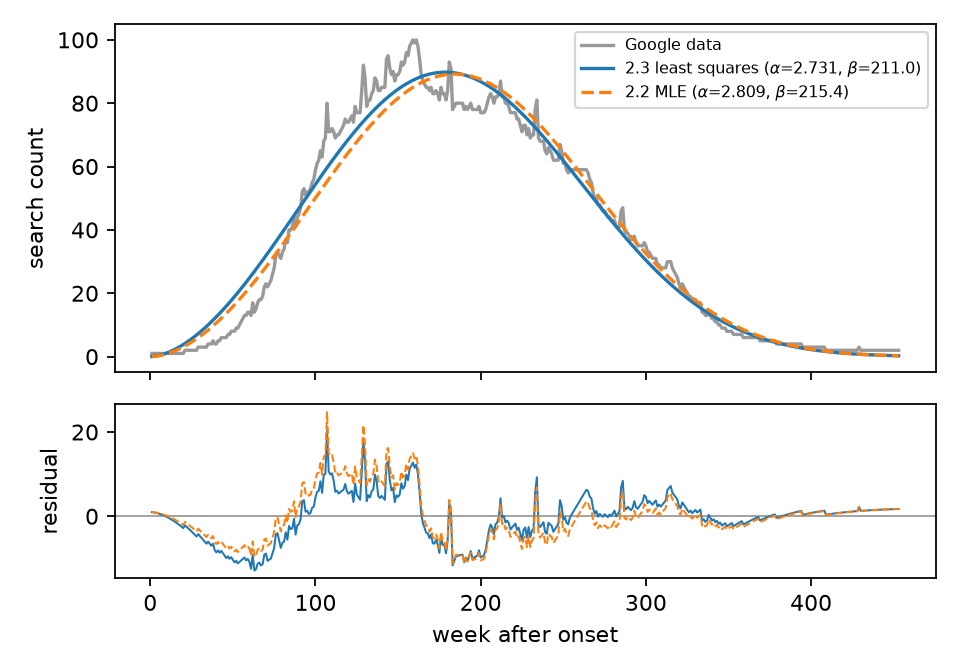
\includegraphics[width=\linewidth]{figures/ls_vs_mle.png}
\end{columns}
\end{frame}

\begin{frame}{Takeaways}
\begin{itemize}
\item Same model, different \textbf{criterion} $\Rightarrow$ different ``best'' parameters
\item Least squares on a histogram is a quick \textbf{hack}: it fits a curve, not a distribution
\item Add an amplitude $A$ to compare a pdf with counts; $\hat A\approx\sum_tc_t$
\item Constrained parameters ($\alpha,\beta>0$) need \textbf{bounds}, or the fit produces \texttt{nan}
\item Nonlinear fits need a sensible \textbf{start}; check by restarting elsewhere
\item Next (2.4): a principled fit for count data
\end{itemize}
\end{frame}

\end{document}
